\chapter{Современные представления о методах определения коэффициента переуплотнения}

Территория нашей страны подвергалась и~подвергается влиянию различных климатических, геологических и~других процессов и~явлений.
Немалая часть территории России находилась под воздействием древнего оледенения.
Определенные участки были подвержены трансгрессии и~регрессии моря.
На некоторых территориях произошел эрозионный срез верхней рыхлой части нормально уплотненного массива грунта, после чего, в~кровле пород обнажаются консолидированные отложения нижней его части.
В~связи с~этим образовались толщи пород, испытывающие в~настоящее время напряжения меньшие, чем в~определенный период своего существования.

На протяжении долгого времени в~нашей стране вопрос о переуплотненных грунтах не исследовался, поэтому существует не так много сводов правил и~ГОСТ, касающихся этой темы.
Чего нельзя сказать о других странах. 
В зарубежных стандартах (BS "--- британский стандарт и~ASTM "--- американский стандарт), в~отличии от ГОСТ, больше отражена зависимость деформационных параметров с~характеристиками состояния и~физическими свойствами грунтов.


В зарубежной механике грунтов широко используются понятия нормально уплотненных и~переуплотненных грунтов, которые различаются по своим деформационным свойствам (Александров С.А. 2018 г.) \cite{aleksandrov2018}.

В нашей стране только в~2019 г. вступил в~действие ГОСТ 58326-2018 \cite{gost58236}, поэтому эта тема новая и~достаточно неизученная.

Как говорилось ранее, изучение параметров, характеризующих предварительное напряженное состояние грунта, чрезвычайно важно при инженерно-геологических изысканиях.
В~отечественной литературе и~документах долгое время этот факт оставался недооцененным. Соответственно, вопрос о значимости этих параметров оставался малоизученным до недавнего времени.
Важно упомянуть, что в~своей работе я только поверхностно исследую эту проблему,  касаясь всего нескольких основных вопросов, связанных с~компрессионными испытаниями, методами обработки полученных данных, а~также их сравнением.

Представим историю существования некоторого сформировавшегося осадка. 
Коэффициент пористости, который характерен для данного осадка сразу после его формирования, называется седиментационным коэффициентом пористости. 
По мере увеличения толщи грунта будет происходить его уплотнение, под действием напряжений от вышележащих слоев.
Осадок будет уплотняться по линии <<нормального уплотнения>> или ветви первичной компрессии. 
В течение существования данного осадка возможна ситуация, когда напряжение будет снижаться, например, вследствие процесса выветривания, перемещения толщ грунта или появления и~последующие исчезновения дополнительных нагрузок, создаваемых ледником. 
При этом будет наблюдаться некоторое разуплотнение осадка, однако, оно не будет соответствовать ветви главного или первичного нагружения, потому что грунт является пластической средой и~большая часть накопленных деформаций является необратимыми. 
Точка при которой происходит разгрузка называется точкой исторического давления. 
Если впоследствии нагрузка на данный грунт снова начнет увеличиваться, то сжатие будет происходить по ветви повторного нагружения до тех пор, пока не дойдет до точки исторического давления, а~далее снова <<пойдет>> по главной ветви или по ветви первичного нагружения. 
Участок от точки начала повторного нагружения до точки пересечения с~ветвью первичной компрессии не является прямой, из-за чего будет явное несоответствие между точкой начала рекомпрессии и~точкой пересечения повторной нагрузки и~ветви первичной компрессии. 
Эта разница и~привела к~тому, что ученые всего мира начали искать методы, исключающие эту погрешность.

Одним из первых, кто ввел понятия <<нормально уплотненные грунты>> и~<<переуплотненные грунты>> был австрийский и~американский геолог и~инженер-строитель Карл Терцаги.

 Под \textit{нормально уплотненными} грунтами Терцаги имел ввиду грунты, находящиеся под нагрузкой бытового давления.
 \textit{Переуплотненный} же грунт, по его мнению, называется грунт, который при своем естественном образовании находился под действием эффективных природных давлений, которые были больше, чем действующее в~настоящее время бытовое давление (Терцаги,~1933) \cite{terz1933}.

Из ранних исследований профессора Карла Терцаги по механике уплотнения мелкозернистых грунтов можно сделать вывод, что зависимость между соотношением пустот и~давлением для первичного или вторичного разветвления кривой сжатия может быть выражена логарифмически. 

Обширные испытания показали, что такое логарифмическое отношение справедливо по крайней мере до 2~МПа, то есть для всего диапазона нагрузок, которые используются в~гражданском строительстве.
Любые существенные отклонения между кривой сжатия ненарушенного глинистого образца, по-видимому, вызваны вариациями нагрузки, которую испытывает грунт в~геологической истории, и~при его удалении из массива.
Это можно определить, исходя из формы кривой разгрузки и~повторного сжатия, полученной при нагружении образца в~условиях, значительно превышающих напряжение, которое испытывал образец грунта, находясь в~массиве.
Нагрузка снижается до нуля, потом снова постепенно увеличивается до еще большей нагрузки (Cazagrande,~1936) \cite{casagrande1936}.

 Опыты профессора Терцаги показали, что для водонасыщенных маловодопроницаемых глинистых грунтов каждому увеличению нагрузки соответствует определенное изменение влажности. 
 Зависимость влажности от нагрузки можно изобразить в~виде кривой,
 которая называется компрессионной. 
 Между влажностью и~коэффициентом пористости у полностью водонасыщенных грунтов существует связь, поэтому компрессионную кривую можно построить как график зависимости давления от коэффициента пористости (Терцаги,~1933) \cite{terz1933}.



 Если изобразить компрессионную кривую в~полулогарифмическом масштабе, 
 тогда изменение коэффициента пористости будут линейно зависеть от логарифма изменения приложенной нагрузки (рис. \ref{fig:comparation}).

 \begin{sidewaysfigure}[p]
  %\begin {sideways} 
  \label{fig:comparation}
  \centering
  \small
  \input{images/comparation.pdf_tex}
  \caption{Сравнение компрессионой кривой в~линейном и~логарифмическом масштабе (Casagrande, 1936) \cite{casagrande1936}}
  %\end {sideways} 
 \end{sidewaysfigure}


 Уравнение компрессионной кривой в~этом случае будет выглядеть следующим образом:
 
 \begin{equation}
 e_i=e_0-C_c \log \left( \frac{\sigma_i}{\sigma_0} \right)
 \label{eq:ke}
 \end{equation}
 
 Индекс компрессии $C_c$ "--- есть тангенс угла наклона полулогарифмической кривой к~оси давлений. Он численно равен разности коэффициента пористости при давлении на данной ступени нагрузки 0,272~МПа и~при начальном давлении 0,100~МПа. Этот коэффициент дает характеристику сжимаемости грунтов в~большом диапазоне давлений. 
 
 Профессором Терцаги был сформулирован закон, который имеет особо важное значение в~механике грунтов и~кладется в~основу установления ряда ее фундаментальных положений: 
 принципа линейной деформируемости, 
 принципа гидроемкости, 
 дифференциального уравнения консолидации и~прочих.
 Этот закон называется <<закон уплотнения грунтов>> и~формулируется так: <<Бесконечно малое изменение относительного объема пор грунта прямо пропорционально бесконечно малому изменению давления>> (Цытович,~1983, с.~36)\cite[36]{cytovich1983}.

 Индекс рекомпрессии $C_r$ "--- тангенс угла наклона части компрессионной кривой в~осях коэффициент пористости "--- логарифм давления.
 Для переуплотненных грунтов выполняются зависимости:% (\ref{eq:over}):

\begin{subequations}
  \label{eq:over}
  \begin{align}
    \label{eq:cr}
    & e_i = e_0 - C_r\log \left(\frac{\sigma_i}{\sigma_0}\right), \quad &\text{при } \sigma_i<\sigma_p \\
    \label{eq:crcc}
    & e_i = e_0 - C_r\log \left(\frac{\sigma_p}{\sigma_0}\right) - C_c\log \left(\frac{\sigma_i}{\sigma_p}\right), \quad &\text{при } \sigma_i>\sigma_p
  \end{align}
\end{subequations}



 
 Артур Казагранде (1902"---1981) "--- американский инженер-строитель австрийского происхождения, внесший значительный вклад в~области инженерной геологии и~геотехники. 
 
 Метод Казагранде был предложен Артуром Казагранде в~1936 году.
 Он стал одним из основных и~самых распространенных методов определения давления предварительного уплотнения, который имеет широкое распространение и~в настоящее время (Труфанов, 2014) \cite{truf2014}.
 
    

 Это графический метод, который основан на определении точки максимальной кривизны на графике компрессионной кривой, построенной в~полулогарифмическом масштабе "--- зависимость коэффициента пористости или относительной деформации от логарифма вертикального (эффективного) напряжения \ref{eq:caz}. 
 Через эту точку проводится касательная к~участку кривой, расположенному за точкой перегиба и~горизонтальная линия. 
 Через угол, который образуют эти две прямые проводится биссектриса. 
 Далее находится точка пересечения биссектрисы угла и~«продолжения» прямолинейного участка компрессионной кривой. Проекция точки пересечения на ось напряжений, есть величина давления предварительного уплотнения. 

 \begin{figure}[ht]
  \centering
  \small

  \input{images/cazagrande-original36+.pdf_tex}
  \caption{Графические построения по методу Казагранде (Casagrande, 1936) \cite{casagrande1936}}
  \label{eq:caz}
\end{figure}


Несколько иной способ обработки данных был предложен Д. Беккером. 

Метод Беккера относится к~группе энергетических методов.
Исторически одним из первых энергию деформация для определения напряжения предуплотнения стал использовать Tavenаs в конце семидесятых годов двадцатого века. В своих работах он опирался на уравения, предложенными Jaeger в 1969 году (Tavenas,~1979)~\cite{tavenas1979}.

Д. Беккер представил свой метод совместно с Jefferies в 1987 году (Jefferies et al, 1987)\cite{jeff1987}.

Согласно методу Беккера значение $\sigma_p$ находится по графику зависимости увеличения работы на единицу объема (произведения давления на деформацию) от приращения вертикального давления. 
Сама процедура определения начинается с~вычисления изменение работы на единицу объема для каждого приращения деформации. 
Далее строится график зависимости работы $W$ от вертикального давления $\sigma$ (рис. \ref{eq:beck}). 
Напряжение в~точке пересечения двух прямолинейных участков, 
которые получаются после данной зависимости, 
и~будет соответствовать давлению предварительного уплотнения (Becker, 1987)\cite{becker1987}.

\begin{figure}[ht]
  \centering
  \small
  %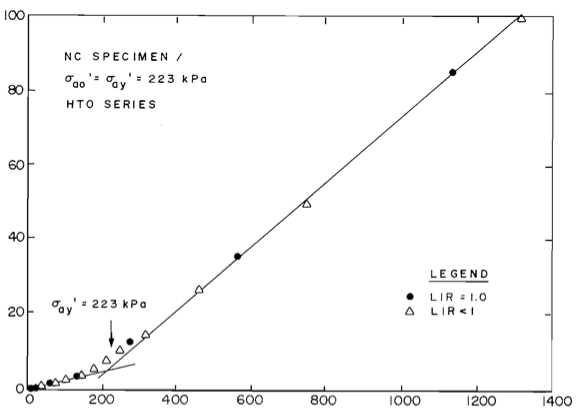
\includegraphics[scale=0.5]{4.png}
  \input{images/becker.pdf_tex}
  \caption{Графические построения по методу Беккера (Becker D.E., 1987) \cite{becker1987}}
  \label{eq:beck}
\end{figure}


%Для повышения надежности определения параметров переуплотнения обработка результатов испытаний производилась двумя наиболее известными способами "--- по методу Казагранде и~методу Беккера, что исключало возможные погрешности, связанные с~неточностью построений. <<Высотные здания, 2016>>
